\section{Определение языка спецификаций}\label{lang_spec}




Вдохновением данной работы послужила статьи~\cite{Palmgren} и~\cite{isaev}. Поэтому сам язык спецификации выглядит как язык описания алгебраических теорий\footnote{Алгебраическая теория это \textit{сигнатура} --- множество сортов и функциональных символов над ними --- и набор аксиом --- множество уравнений над термами, построенными с помощью типизированных переменных и функциональных символов. Сами функциональные символы тотальны, то есть применимы ко всем представителям данных сортов}.

А именно, помимо правил вывода у нас есть сорта и функциональные символы. Каждая конструкция в языке --- это функциональный символ в логике, а правила вывода и редукции --- это аксиомы. Правила вывода говорят, когда некоторый функциональный символ определен. Все функциональные символы являются частичными функциями, поэтому это существенно алгебраические теории, а не просто алгебраические. Частичные потому, что например конструкция if-then-else в качестве первого аргумента принимает только терм типа Bool, иначе она не определена и проверка типов должна уведомлять пользователя о некорректности сформированного терма.

Начнем с примера описания языка с зависимыми типами~(рис.\ref{lpi})~\cite[Глава~2.1]{book:pierce}

\begin{figure}
    \centering
	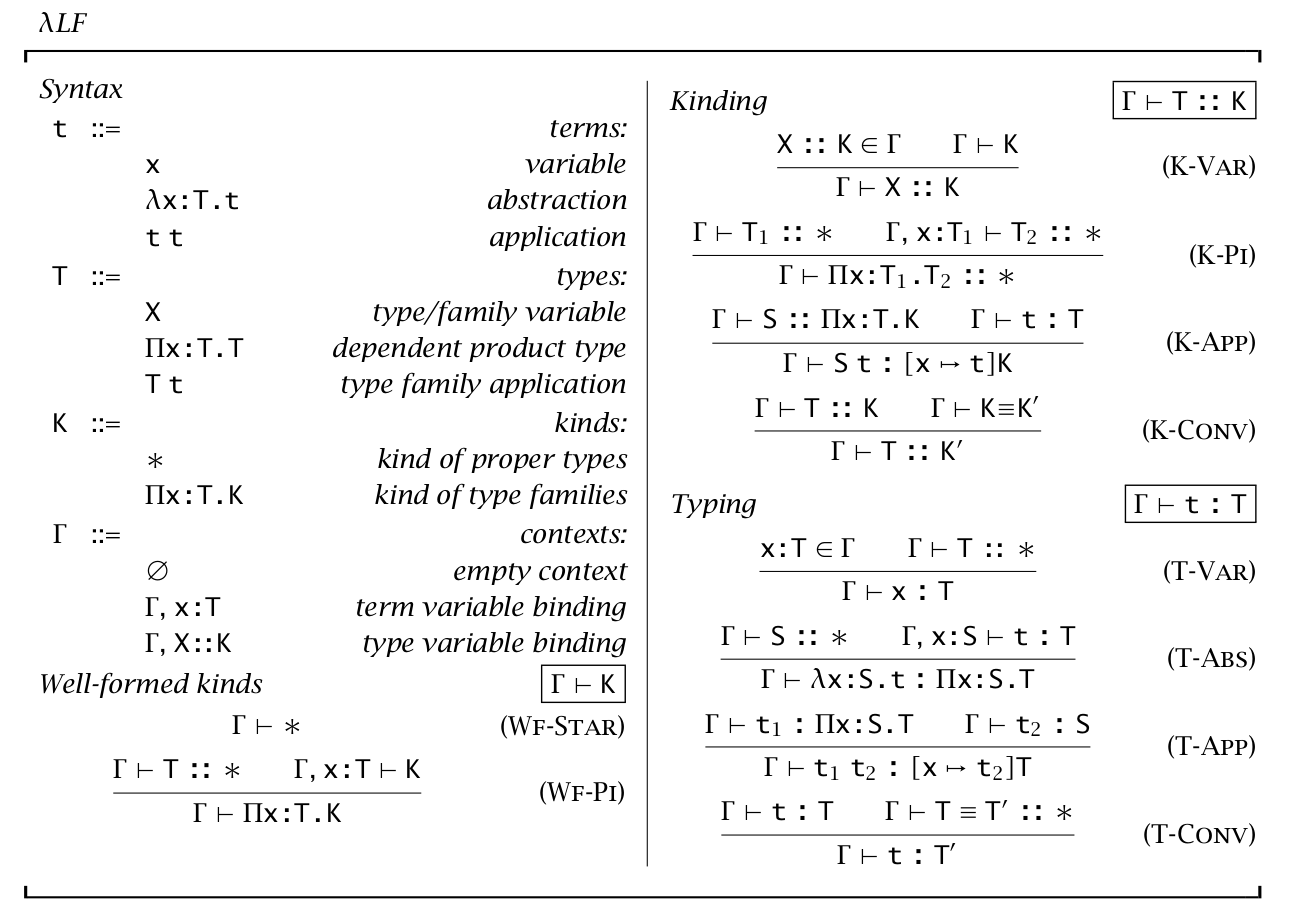
\includegraphics[scale=0.35]{img/lp.png}
	\caption{Язык с лямбдой и $\Pi$-типами }
	\label{lpi}
\end{figure}

В этом языке явно выделяются три сорта (можно думать о сортах как о метатипах): виды, термы и типы (правила связанные с видами и само их описание опущены для простоты).

Также явно выделяются примитивы языка (в дальнейшем мы называем их функциональными символами):
абстракция, $\Pi$-типы (функции в языках с зависимыми типами) и аппликация. Легко заметить, что во всех яхыках присутствуют подстановка, контексты, символ `:' означающий, что тип терма слева есть терм справа, и связывание переменных.

Правила вида T-Conv и T-Var всегда верны в зависимых языках, поэтому у нас они есть по умолчанию. Также подразумевается рефлексивность, симметричность, транзитивность и конгруэнтность равенства.

Если принять во внимания все наблюдения выше, то так этот язык будет выглядеть в нашем языке спецификации\footnote{Важно понимать, что запись $\_ \vdash$ не означает, что контекст пуст, если слева ничего не написано, это эквивалентно записи $\Gamma \vdash$.}:

\begin{lstlisting}[frame=single]
DependentSorts:
  tm, ty
FunctionalSymbols:
  lam: (ty, 0)*(tm, 1) -> tm
  app: (tm, 0)*(tm, 0)*(ty, 1) -> tm
  pi : (ty, 0)*(ty, 1) -> ty
Axioms:
  K-Pi =
    forall T1 : ty, x.T2 : ty
      x : T1 |- T2 def |--- |- pi(T1, x.T2) def
  TAbs =
    forall S : ty, x.T : ty, x.t : tm
      x : S |- t : T |--- |- lam(S, x.t) : pi(S, x.T)
  TApp =
    forall t1 : tm, t2 : tm, S : ty, x.T : ty
            |- t1 : pi(S, x.T),
            |- t2 : S,
      x : S |- T def
      |--------------------------
      |- app(t1, t2, x.T) : T[x:=t2]
Reductions:
  Beta =
    forall x.b : tm, A : ty, a : tm, z.T : ty
       |--- |- app(lam(A, x.b), a, z.T) => b[x:=a] : T[z:=a]
\end{lstlisting}

Типизирование метапеременных позволяет проверять правильность применения функциональных символов и наличие нужных переменных в контексте. Именованные переменные служат для определения порядка переменных в контексте и не несут какой-то дополнительной информации.

Также в язык была добавлена проверка на c-стабильность --- можно помечать аксиомы типами, тогда аксиома применима, только если все переменные входящие в терм являются представителями этих типов. Если список типов пуст, то производится проверка терма на отсутствие свободных переменных.

\subsection{Ограничения на спецификации, налагаемые языком}\label{constraints}

Если не налагать никаких ограничений на спецификации, то пользователь может написать спецификацию, для которой мы не сможем сгенерировать функцию проверки типов. Поэтому вводятся следующие ограничения на спецификации языков:

\begin{enumerate}
\item Запрещено перекрытие переменных, которые уже есть в контексте. Это чисто стилистическое ограничение, которое не вносит никаких ограничений на сами языки.

\item Запрещено равенство в заключении правил вывода, они заменены редукциями.

\item \label{funsym_concl} В заключении правила вывода может быть только конструкция языка с метапеременными в качестве аргументов. Не должно быть подстановок или метапеременных на верхнем уровне слева от отношения типизации. Неясно как работать с подстановками в заключениях правил вывода, так как на этапе проверки типов знание того, что ``нам передается что-то с выполненной в него подстановкой куда-то'', не дает нам никакой дополнительной информации, в сравнении с отсутствием этого знания. Также неясно, что делать с метапеременной переданной в заключении, так как она будет подходить подо все выражения сорта этой метапеременной. Поэтому разрешены только конструкции языка в заключении.

\item Все аргументы в конструкцию языка в заключении правила вывода должны быть метапеременными --- случай содержащий не только метапеременные требует дальнейшего исследования. Метапеременные должны быть с теми же контекстами, что и в forall --- если бы контексты были шире, то в алгоритме проверки типов сразу же приходилось бы проверять выражения, соответствующие метапеременным, на возможность удаления лишних переменных.

\item \label{one_per_fun} Правило вывода для каждой конструкции всегда одно, иначе появляется недетерминированность в проверке типов --- неясно какое правило вывода выбрать при проверке типов. В ходе эксплуатации не возникало нужды в обратном. Понадобилось бы более тщательное обдумывание последствий отсутствия данного ограничения. В будущем возможны изменения.

\item В заключении контекст не должен быть расширен --- это ограничение связано с тем, что иначе смысл правила вывода становится странным. А именно: конструкция применима только при введении переменных в контекст.

\item Если в заключении правила вывода написана конструкция возвращающая сорт термов, она обязана быть проаннотирована типом (нельзя просто написать $ \vdash f(\ldots)\ def$). Так как иначе становится неясно какой тип возвращать при выводе типа данной конструкции.

\item Подстановки разрешены только в метапеременные --- в принципе, это слабое ограничение, которое облегчает жизнь при реализации, не ограничивая пользователя. Нам, как разработчикам, не нужно ещё и на уровне мета-языка (языка спецификации) заботиться о подстановках.

\item \label{tm:Meta} Все метапеременные, используемые в предпосылках, должны либо присутствовать в метапеременных заключения, или же должны быть типами какой-либо предпосылки. Иначе попросту неясно откуда брать выражения, соотвествующие этим метапеременным, при проверке типов языка.

\item \label{def_metas} Если в заключении правила вывода во вводимой конструкции языка встречаются метапеременные с контекстами $x_1 \ldots x_k . T$, то должна существовать предпосылка вида $x_1 : S_1 \ldots x_k : S_k  \vdash T$ в правиле вывода конструкции. Это сделано для того, чтобы не передавать типы контекстов метапеременных в конструкции явно, а выводить их из такого рода предпосылок. Предпосылки такого вида мы называем \textit{определениями метапеременной}.

\item \label{right::} Если метапеременная является типом предпосылки и не встречается в аргументах конструкции, то она может использоваться только справа от двоеточия. Таким образом избегаются ситуации связанные с порядком проверки предпосылок языка. А именно: если у нас есть $x : S \vdash t : T,\ x:T \vdash r : S$, то нужно строить граф зависимостей для предпосылок и использовать порядок полученный в результате его топологической сортировки в генерации кода (Аналогично с~\ref{toposort}). Так как иначе нам неоткуда будет взять выражение соответствующее этой метапеременной при проверке типов.

\item \label{order:Meta} Все переменные контекстов определения метапеременных (то есть предпосылки, описанные в Пункте~\ref{def_metas}) могут использовать только метапеременные, переданные левее внутри конструкции в заключении, --- это связано с тем, что иначе могут возникнуть циклы в определениях метапеременных: S тип с аргументом типа R, R тип с аргументом типа S, S тип с аргументом типа R и т.д. А

\item Из-за ослабления условия на метапеременные в Пункте~\ref{tm:Meta}, порядок метапеременных неочевиден. Решение данной проблемы и~(\ref{order:Meta}) описано в Разделе~\ref{toposort}.

\item Редукции не учитывают предпосылок при приведении в нормальную форму --- предполагается что они не конфликтуют с правилами вывода и проверок корректности выражений в правилах вывода достаточно.

\item В редукциях все метапеременные справа от `\lstinline{=>}' должны встречаться и слева от него. Иначе непонятно откуда взять выражения соответствующие этим метаперемнным при формировании правой части редукции.

\item Подстановка запрещена слева от `\lstinline{=>}'. Это сделано для возможности сопоставления с образцом при генерации функции приведения в нормальную форму. Также как и в Пункте~\ref{funsym_concl} не очень понятно, как восстанавливать исходную метапеременную до подстановки.

% \item Все редукции всегда стабильны. В ходе эксплуатации не возникало нужды в обратном.

\end{enumerate}

\subsection{Проверки корректности спецификации языка}

Все ограничения выше проверяются при обработке спецификации языка.

Также тривиальными проверками, осуществляемыми после синтаксического разбора языка, являются:
\begin{itemize}
\item Все метапеременные, используемые в правилах вывода/редукциях находятся в контексте, включающем их контекст, описанный в подразделе forall.
\item Проверка того, что сорты используемых выражений совпадают с сортами аргументов конструкций.
\item Подстановка осуществляется в переменные, которые есть в свободном виде в метапеременной.
\item Контексты метапеременных содержат все их переменные.
\item Все конструкции языка имеют ассоциированное правило вывода.
\end{itemize}

